\section{Conception}

\todoGeneric{10 à 15 pages de conception}

\todoGeneric[inline]{Intro de la section conception}

\subsection{Robot}

\subsubsection{Électronique}
\todoWho{Jordan}

Puisque la méthode de lancer choisi est la roue d’inertie et la méthode de chargement est avec un pignon et une crémaillère, nous devions intégrer au montage un moteur DC et un servomoteur.
Ainsi le moteur choisi pour faire tourner la roue d’inertie servant à propulser la balle est un moteur DC sans balai.
Nous avons opté pour ce type de moteur puisque le nombre de rotation par minute devait être suffisamment élevé pour propulser la balle assez loin et le torque devait également être suffisamment important pour éviter une obstruction lors du passage de la balle.
L’un d’entre nous possédait chez lui un moteur pouvant servir au projet, c’est donc lui qu’on a utilisé.
Il s’agit du moteur TrackStar 8.5T.

\todo[inline]{add image}

Puisque c’est un moteur sans balai, il ne suffit pas seulement d’appliquer une tension à ses bornes pour qu’il tourne.
Nous avons donc acheté un contrôleur servant à faire tourner le moteur et à modifier la vitesse grâce à un signal d'entrée.
Le contrôleur choisi est le ESC 30A.
Ce contrôleur a comme entrées une alimentation qui doit être d’environ 7,4~V pour que le moteur fonctionne comme il se doit selon la fiche technique du moteur \cite{noauthor_trackstar_nodate} et trois autres fils qui doivent être branché sur l’Arduino.
Ces trois fils doivent être branché au commun de l’Arduino, au 5~V et à une sortie pouvant produire un PWM soient les pins 2 à 13 de l’Arduino Mega.
Les trois fils de sorties du contrôleur sont branchés directement sur les trois fils du moteur.
Pour ce branchement il a été très important de vérifier que le commun de l’alimentation soit connecté au commun de l’Arduino.

\todo[inline]{add image: Circuit d'alimentation et de contrôle du moteur DC sans balai}

Par ailleurs, le moteur doit recevoir une tension d’alimentation de 7,4~V comme indiqué sur la figure\todo{make ref to figure}.
Cependant, les seules prises d’alimentation sur le robot pouvant fournir un gros courant sont des prises de 5 V et 12 V.
Ainsi, nous avons acheté un régulateur de tension de type buck pour pouvoir passer de 12~V à 7,4~V.
Le régulateur de tension acheté est le VMA404 utilisant un LM2596, car c’était un modèle peu dispendieux disponible à la boutique Electro5 à Sherbrooke.
Comme indiqué dans la prochaine figure\todo{Add ref to figure}, la tension d’entrée est de 12~V et en mesurant la tension de sortie avec un multimètre nous pouvons ajuster le potentiomètre pour avoir 7,4~V en sortie.

\todo[inline]{add image: Régulateur de tension VMA404}

Pour ce qui est du servomoteur, ce dernier est branché directement dans l’un des ports d’entrée sur la carte Robus conçu à cet effet.

Ensuite, pour la communication Bluetooth, nous avons acheté le module HC-05, car c’était celui qui avait était suggéré par le technicien Serge lors du séminaire sur les capteurs.
Son branchement est effectué comme à la prochaine figure\todo{Add ref to figure}.

\todo[inline]{add image: Circuit de branchement du module Bluetooth HC-05}

On voit donc sur la figure \todo{Add ref to figure} que le module a 4 fils de branchement.
Il y a deux fils pour l’alimentation, et deux fils pour la réception et la transmission du signal.
Le module marche à des tensions de 3,3~V c’est pourquoi il y a le diviseur de tension à l’entrée RXD du module suggéré sur le site \cite{noauthor_setting_nodate}.
L’alimentation est toutefois branchée au 5~V, car il y a un régulateur interne sur le module Bluetooth pour passer de 5~V à 3,3~V.

\subsubsection{Logiciel}
\todoWho{Thierry}

\todo[inline]{add pseudocode}

\todo[inline]{add Diagramme d’activité}

La programmation du robot peut sembler compliqué, mais en réalité elle était très simple.
L’application Android qui est conçue pour communiquer avec le robot envoie un chiffre en fonction de l’action que veut faire l’utilisateur.
Par exemple, si l’utilisateurs appuie sur la balle pour tirer, le téléphone va communiquer avec le récepteur Bluetooth du robot en lui envoyant le chiffre 6.

\todo[inline]{add image}

Le chiffre envoyé est de type «char».
Pour simplifier la compréhension du code, nous avons initialisé chacune des constantes et avons attribué une variable représentative.
La \todo{insert reference (maybe figure)} représente chacune des constantes qui ont été initialisé.
Ensuite, lors de la configuration de l'Arduino, le Bluetooth est initialisé avec les pins correspondantes.
De plus, le moteur sans balai que nous avons utilisé est configuré comme un servo moteur, donc nous avons utilisé la classe MegaServo pour initialiser ce moteur.
Les valeurs à rentrer en paramètre de la fonction ne sont pas des angles puisque c’est un moteur sans balais.
Selon \cite{arduino_arduino_nodate} le contrôleur du moteur reçoit une impulsion entre 1000~$\mu$s et 2000~$\mu$s, c’est pourquoi nous utilisons ces valeurs.
Dans ce cas, 1000 représente la valeur minimum c’est-à-dire que le moteur ne tourne pas, alors qu’à 2000, le moteur tourne à sa pleine capacité.
Le servo moteur a été configurer avec la libraire LibRobus, qui nous a été offerte.

La boucle vérifie à chaque fois si l’application a envoyé un message.
Lorsqu’un message est reçu, l’Arduino exécute l’action demandé.
L’action d’avancer et de reculer est très simple, elle consiste uniquement à configurer les 2 moteurs à 0,2~V pour avancer et à -0,2~V pour reculer.
Nous avons jugé que l’utilisation du PID pour cette fonction n’était pas nécessaire, puisque le robot ne fait que de très petits mouvements.
Ensuite, lorsque l’utilisateur relâche le bouton, un second message est envoyé au robot pour configurer les 2 moteurs à 0~V (les arrêter).

Les trois prochaines conditions sont reliées au canon du robot.
Lorsque l’utilisateurs demande un incrément de la vitesse du moteur, la variable forceMoteur est incrémentée de 5.
Pour la condition où le joueur demande une décrémentation, la vitesse du moteur est décrémentée par 5.
Pour la distance que nous désirions des verres, après quelques tests, nous avons réalisé que la vitesse optimale était entre 1150 et 1200.
C’est pourquoi les 10 niveaux de forces du moteur se situent entre 1150 et 1200.
Ensuite, lorsque le joueur appuie sur tirer, l’Arduino reçoit comme commande de tirer.
L’angle du servo moteur est donc configurer pour reculer à son minimum, et retourner à son angle initial de 180 degrés.
Durant cette action, le moteur sans balai part sa puissance à la vitesse demandée par l’utilisateur.
Donc, lorsque la balle est poussée dans la roue de mousse reliée au moteur sans balai, la balle est propulsée et l’Arduino envoie comme message de fermé le moteur DC.
Au départ, nous voulions laisser le moteur sans balai rouler en tout temps, cependant par souci d’économie d’énergie et pour que le système soutenant le moteur s’use moins rapidement, nous avons décidé de le partir uniquement lorsque l’Arduino reçoit la commande de tirer.

\subsubsection{Mécanique}
\todoWho{Will}

Le lanceur de balles est une partie très importante du projet,
car il doit être capable de faire ce qu’il est conçu de façon consistante pour faciliter son utilisation.
Il se sépare en 3 parties principales:
la partie propulsion,
la partie recharge ainsi que
la partie visé.

\subsubsection{Mode de propulsion}
Pour la propulsion de la balle, trois systèmes ont été étudiés pour assurer une certaine précision tout en gardant le système simple.

\paragraph{Option 1: par contact}
Nous avons pensé à un système comprimant un ressort à l’aide d’un boîte de vitesse et d’une crémaillères.
Ce système à vite été écarté puisque nous ne savions pas si les pièces, principalement imprimées en PLA, allaient être capable de supporter l'énergie emmagasinée dans le ressort.
De plus, il aurait fallu avoir une façon de placer les balles à la bonne distance du ressort et les faire tenir en place avant le contact, ce qui aurait compliqué les choses rapidement.
Un solénoïde à aussi été envisagé pour frapper la balle, mais nos connaissance en magnétisme n’étaient pas adéquates pour considérer cette option plus sérieusement.

\todo{(Placer photo croquis)}

\paragraph{Option 2.1: par piston}
Un système comparable à ce que l’on retrouve dans les jouets de type “Airsoft” à aussi été étudié.
Ce système consiste encore une fois à comprimer un ressort attaché à un piston pour créer une différence de pression entre le devant et le derrière de la balle, la propulsant vers l’avant.
Ce système comporte les mêmes désavantages que la première option, en plus des problèmes d’étanchéité que peuvent apporter les pièces imprimées.
Il a donc été écarté.

\paragraph{Option 2.2: par air comprimée.}
Nous avons pensé à remplacer le piston par une pompe à air et un réservoir pressurisé.
Sachant que l’air comprimé peut être très dangereux si le système échoue, et que nous allions être en présence de famille lors des démonstrations, cette option était donc une mauvaise idée.
De plus, un système comme celui-ci aurait été beaucoup plus compliqué que le système final choisi.
\todo{(Placer photo croquis)}

\paragraph{Choix final: Roue d’inertie.}
Nous avons donc opté pour une roue d’inertie pour propulser nos balle.
L’idée est venue des jouets de la marque NERF, qui utilisent 2 roues tournant en sens inverse pour propulser des fléchettes de mousse sur une distance acceptable.
Ce système est aussi assez simple, puisqu’il requiert seulement un moteur pouvant tourner à une vitesse contrôlable et d’une roue d’inertie.
Dans les lanceurs NERF, les roues étaient en plastique dur, puisque que les projectiles étaient en mousse molle et très malléable.
Dans notre cas, nous ne voulions pas briser la balle, il a donc fallu rajouter une extérieure de mousse servant à isoler les cadres de portes.

\todo{(Placer photo de la roue)}

\subsubsection{Méthode de chargement de la balle}
Quelques méthode pour pousser les balles vers la roue d’inertie ont étés envisagées.
Voici les trois options principales.

\paragraph{Option 1: Par gravité}
Nous avons pensé à utiliser la gravité pour pousser les balles sous la roue d’inertie pour simplifier le système.
ce système aurait seulement eu besoin d’un servo pour assurer qu’une seule balle tombe à la fois dans le lanceur.
Cependant, le système de roue d’inertie fait que la distance entre la roue et la base du lanceur est plus petit qu’une balle (pour que la balle soit pressée dans la mousse, assurant un transfert d’énergie suffisant pour la propulser.
La gravité n’avait donc pas la force nécessaire pour enfoncer la balle sous la roue.

\paragraph{Option 2: came et tige-poussoir.}
Nous voulions nous servir d’un servo pour gérer le chargement, car ils sont simple à utiliser et assez précis pour nos besoins.
Le débattement nécessaire pour amener les balles de la position ou les balles sont placées jusqu’en dessous de la roue est d’environ 75 mm (les balles faisant 40mm de diamètre et en ajoutant quelques millimètres pour assurer la solidité du lanceur).
Les servos allant seulement de 0 à 180 degrés, il aurait fallu une camme d’au moins 75 mm de diamètre pour accommoder ce débattement, ce qui aurait été beaucoup trop gros en comparaison au lanceur.

\paragraph{Option 3: pignon et crémaillère}
Cet option est parfaite, puisqu’elle règle le seul problème que la came avait: la dimension des roues.
En se servant des CADs fournies par McMaster.com, il a été facile de trouver des pièces de dimensions adéquates pour notre système.
Un pignon ayant un diamètre primitif de 1 pouce ayant 20 dents et sa crémaillère répondaient parfaitement à nos critères de dimensions.
Il nous faudrait donc faire tourner le pignon une fois(2*pi*0,5 po) pour atteindre le débattement voulu (3po).
Il fallait donc changer 180 degrés du servo en 360 degré.
Nous avons donc utilisé deux roues ayant le même diamètre primitif que la première, dont une avait 2 fois plus de dents pour assurer un tour complet.
Les roues de 12 et 24 dents ont donc étés choisies car elles etait de bonne dimensions.

\begin{figure}[h!]
    \centering
    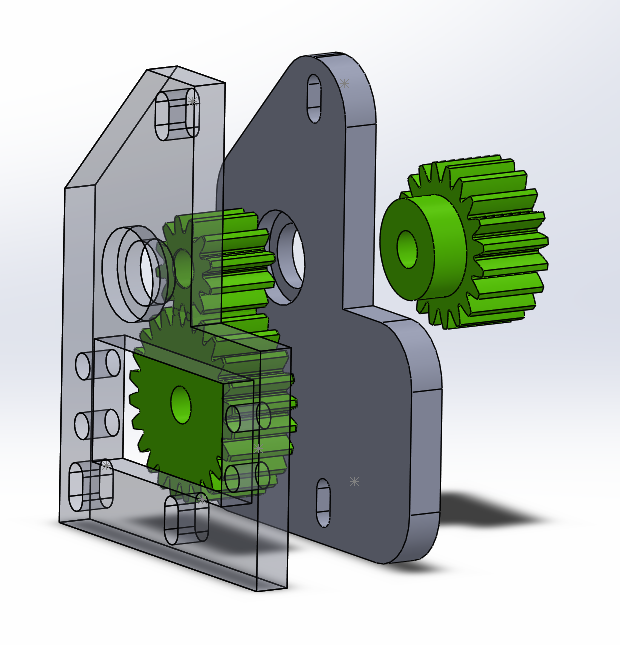
\includegraphics[width=0.5\linewidth]{img/s2/cad/gearbox1}
    \caption{Description de l'image.}
    \label{fig:s2-cad-gearbox1}
\end{figure}
\todo{add a description to the figure}

\subsubsection{Mode de visé}
Plusieurs options s’offraient à nous pour visé avec le lanceur.
La première étant de jouer avec l’angle du lanceur pour aller chercher différentes distance (pour atteindre tous les verres de beer pong).
Cette option a été écartée puisque nous ne savions pas le poids finale du lanceur et si un servo allait être capable de le maintenir en place de façon constante.
Nous avons donc conçue un un support ayant un arc de cercle ce qui nous a permit de choisir une angle et de sécuriser le lanceur à cet angle.

\missingfigure{support de visé}
La distance des lancers allait donc être déterminée par la vitesse à laquelle la roue d’inertie tourne, ainsi que la pression qu’elle applique sur les balles.

\subsubsection{Version finale}
La version finale allait donc être un lanceur fixe rechargé par une crémaillère, qui propulse les balles à l’aide d’une roue d’inertie.
Notre Première itération comportait une grande rampe pour assurer que les balles aient un maximum de temps en contact avec le lanceur pour augmenter la précision.
Cette idée de rampe a été abandonnée lorsque nous avons réalisé de qu’elle ampleur elle devait être pour répondre à nos besoins (un arc de cercle d’environ 150 mm de rayon, pour assurer un arc de cercle assez graduel.
Nous avons donc optés pour un lancer direct avec un petit canon pour réduire les imprécisions de la roue.

\missingfigure{Rampe de lancement}
fig:Rampe de lancement
\begin{figure}[h!]
    \centering
    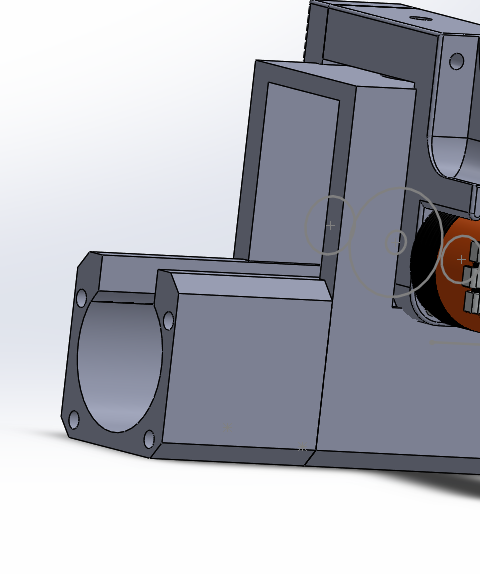
\includegraphics[width=0.5\linewidth]{img/s2/cad/cannon}
    \caption{Description de l'image.}
    \label{fig:s2-cad-cannon}
\end{figure}
\todo{add a description to the figure}

Une autre amélioration de la version finale à été de fixer l’axe de la roue d’inertie des deux côtés et d’ajouter un roulement à bille.
Les pièces imprimées en 3D sont rarement balancées et la roue ajoutait beaucoup de vibration au système.
Le roulement à bille réduisait aussi la friction entre l’arbre de la roue et le support en plastique, qui avait tendance à fondre durant l’utilisation.
De plus, ce support facilitait aussi l’ajustement de la position de la roue d’inertie.
Un écrou sous le support était facilement accessible et nous n’avions plus besoins de défaire le montage au complet pour dévisser le moteur et changer sa hauteur.
Ce support était aussi imprimé en 2 pièces pour faciliter son implémentation au système.

\begin{figure}[h!]
    \centering
    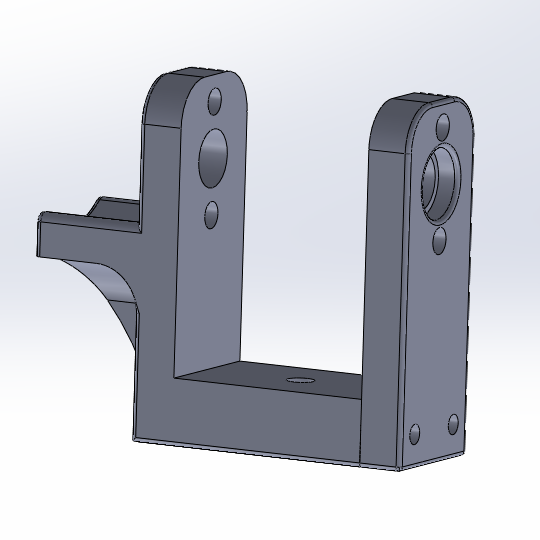
\includegraphics[width=0.5\linewidth]{img/s2/cad/motorholer}
    \caption{Description de l'image.}
    \label{fig:s2-cad-motorholer}
\end{figure}
\todo{add a description to the figure}

\todo{ajouter photo}

Pour assurer un maillage adéquat entre les roues de la boîte de transmission et la crémaillère, des trous oblongs avaient étés utilisés.
Cependant, Nous nous sommes rendu compte que ces trous ne servaient pas à grand chose et que les engrenages devaient être plus contraintes.
La position du servo a aussi été modifiée puisqu’il interférait avec les tiges filetées servant à fixer le système.
Nous avons donc conçue une boîte de transmission complètement indépendante du lanceur et qui gardait toujours la bonne distance entre les engrenages.
Cette boite était par la suite fixée au lanceur à l’aide des trous prévus à cette effet.

\begin{figure}[h!]
    \centering
    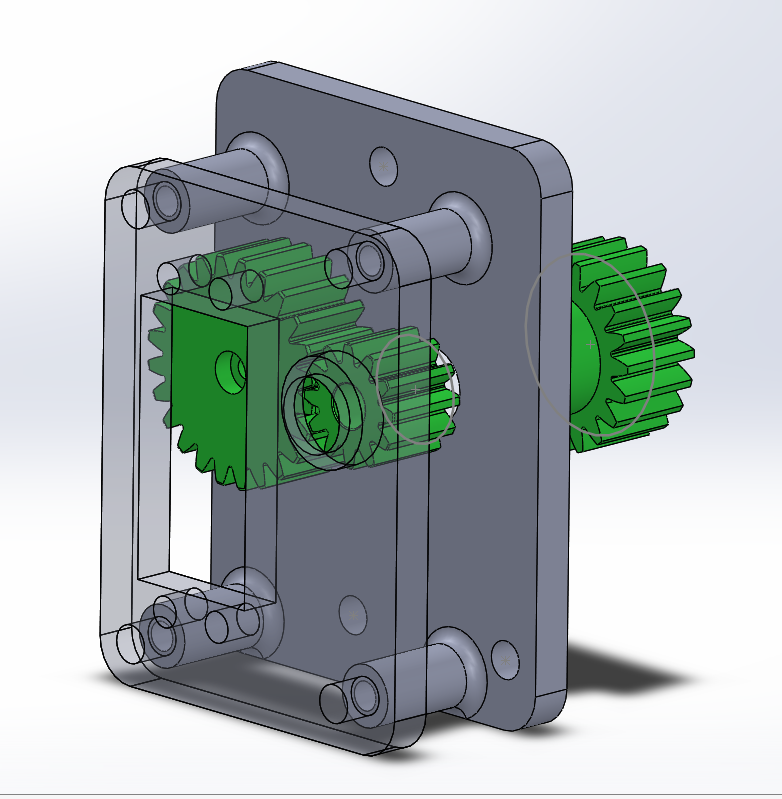
\includegraphics[width=0.5\linewidth]{img/s2/cad/gearbox2}
    \caption{Description de l'image.}
    \label{fig:s2-cad-gearbox2}
\end{figure}
\todo{add a description to the figure}

\todo{ajouter photo}
Le PLA est un plastique malléable et facile à percer.
Nous nous sommes servis de ces caractéristique pour décortiquer notre lanceur en pièces faciles à imprimer et nous avons utilisés des tiges filetées de dimensions 10-32 pour tenir le tout ensemble.

\begin{figure}[h!]
    \centering

    \begin{subfigure}{0.4\linewidth}
        \centering
        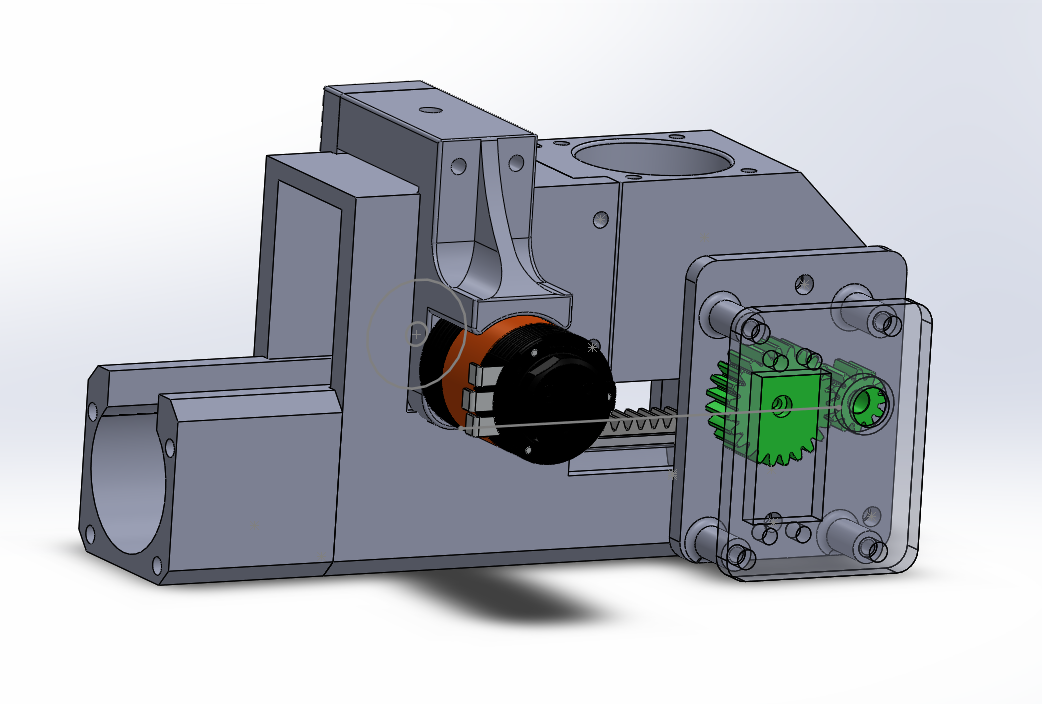
\includegraphics[width=\linewidth]{img/s2/cad/lanceur1}
        \caption{Description de l'image.}
        \label{fig:a1-s2-cad-lanceur1}
    \end{subfigure}
    \begin{subfigure}{0.4\linewidth}
        \centering
        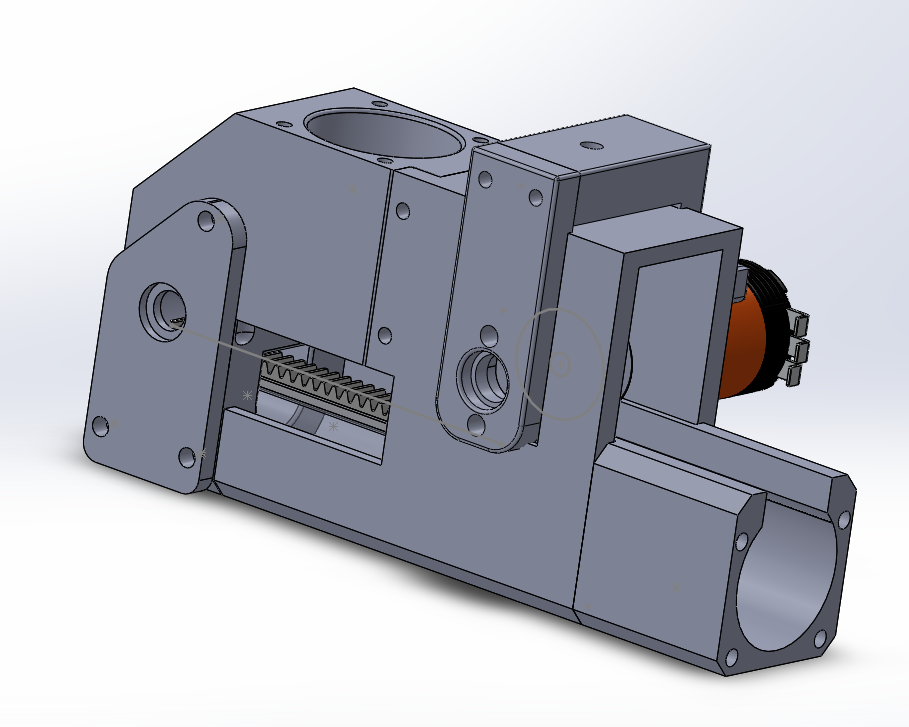
\includegraphics[width=\linewidth]{img/s2/cad/lanceur2}
        \caption{Description de l'image.}
        \label{fig:a1-s2-cad-lanceur2}
    \end{subfigure}

    \caption{Description de l'image.}
    \label{fig:template-example-flottante}
\end{figure}
\todo{add a description to the figure}

\todo{ajouter photo monté}

\subsection{Verre}

\subsubsection{Électronique}
\todoWho{Vincent}

\todoPoints{Vous y joindrez tous les documents nécessaires (croquis, schémas électriques, ordinogrammes, calculs, etc.) pour expliquer vos choix.}
\todoPoints{Justifier vos choix.}
\todoPoints{Mentionner les performances et les limitations du prototype.}

\subsubsection{Logiciel}
\todoWho{Thierry}

\todo{add pseudocode}

\todo{add Diagramme d’activité}

Pour les verres, il fallait programmer le Arduino Mega 2560 qui a été utilisé.
Cette programmation était relativement simple.
Six des entrées digitales (configurées en entrées) de l'Arduino étaient connectées aux verres, ces entrées sont les pins 22 à 32.
Ces entrées sont par incrément de 2, ce qui totalise les six verres.
Six autres entrées digitales (configurées en sortie) étaient connectées aux LEDS, ceux-ci sont les entrées 1 à 7.
Lors de la configuration du Arduino (init), une tension de cinq volts par sorties digitales est envoyé pour allumer les LEDS.
Ensuite, le programme passe à la boucle.
La boucle (loop) vérifie si les verres ont été réussis.
Le programme sait lorsqu'un verre est réussi en vérifiant les entrées digitales 22 à 32.
Lorsque l'entrée ne détecte plus de tension, un message est envoyé pour fermer la LED correspondante.
Les LEDS ont été organisées pour que chaque incrément correspond au bon verre.
Par exemple, la LED 22 est reliée à l’entrée 1, la LED 24 est reliée à l’entrée 2 etc…

\subsubsection{Mécanique}
\todoWho{Vincent}

\todoPoints{Vous y joindrez tous les documents nécessaires (croquis, schémas électriques, ordinogrammes, calculs, etc.) pour expliquer vos choix.}
\todoPoints{Justifier vos choix.}
\todoPoints{Mentionner les performances et les limitations du prototype.}

\subsection{Application}

\subsubsection{Logiciel}
\todoWho{Thierry}

\todoPoints{Vous y joindrez tous les documents nécessaires (croquis, schémas électriques, ordinogrammes, calculs, etc.) pour expliquer vos choix.}
\todoPoints{Justifier vos choix.}
\todoPoints{Mentionner les performances et les limitations du prototype.}
